\documentclass{article}

\title{Evaluating the Relevancy of JFIF Image Compression on the Internet}
\author{Uzen}
\date{Jul 22}

\usepackage{indentfirst}
\usepackage{tabularx,booktabs}
\usepackage[a4paper]{geometry}

\usepackage{amsmath}
\usepackage{tikz}
\usepackage{xcolor}

\usepackage{hyperref}
\hypersetup{%
	linktoc    = all,
	colorlinks = true,
	urlcolor   = blue,
	linkcolor  = black,
	filecolor  = black,
	citecolor  = black,
	pdftitle   = {\@title},
	pdfauthor  = {\@author},
}

\usepackage[backend=biber,style=mla,showmedium=false]{biblatex}
\addbibresource{citations.bib}
\DeclareBibliographyDriver{footcite:online}{%
  \usedriver
    {\renewbibmacro*{bbx:savehash}{}}
    {online}}
\providecommand{\biburldatelong}{}

\usepackage{titlesec}
\newcommand{\sectionbreak}{\clearpage}

\usepackage{caption}
\usepackage{subcaption}

\usepackage{listings}
\usepackage{wrapfig}

\parskip=1em

\begin{document}

\maketitle

{\LARGE \tt this is a DRAFT!!!!!!}

\tableofcontents
\newpage

\section{Introduction}
Compression is the cornerstone of the internet.
Behind the millions of bytes flowing between computers everyday around the world, compression algorithms are behind every single data packet.
Compression algorithms are tools that can seemingly magically shrink a digital document, sometimes until they are a tenth of their size.
Due the many uses of compression algorithms, they have been used in many different fields.
From shrinking large backups for storage to speeding up the transfer of data across the web, compression algorithms are crucial to modern computing.

% too personal here
One specific field that I was interested in was website hosting.
A personal website can be a good representation of themselves, similar to a more polished social media page.
For a period of time, I was quite interested in starting my own website, renting virtual servers from Aliyun to start my project.
However, I quickly ran into an issue.
In the modern times, technology has progressed at an exponential rate, storage and bandwidth speeds are increasing at an extraordinary rate.
It is common to see computers with hundreds of gigabytes of storage and gigabit connection to the internet.
% less personal
So it was quite a surprise for me when I found out that adding bandwidth and storage to my server costed money.
A small, affordable server would only come with 10 to 50 gigabytes of storage a measly 1 megabit bandwidth connection (or purchase bandwidth by the gigabit used).

Due to this limitation, the website I made was slow.
I couldn't upload many images or videos because the server would run out of storage, or make the website load at a snail's pace.
This made me very careful about the files I upload, especially the sizes of image and videos.
My curiosity eventually lead me to image compression.
When an image is stored, there's different file types:\texttt{~.png,~.jpg,~.gif}.
These are actually different methods of storing images, using different methods image compression techniques.
When creating my website, I had to choose what method of image compression to use.
Each different method has its advantages and disadvantages.
% add some conclusion from personal perspective

One format of compression I am very interested in is JFIF compression (commonly found in JPEG files).
JFIF uses a mixture of clever math and the characteristics of the human eye to shrink photos.
It is commonly used in digital cameras.
However, JFIF was originally invented over 30 years ago (August 1990~\autocite{jpeg}), and have not account for the many modern technological advances.
For example, JFIF is bad at dealing with digital art and digital text due to limitation of the compression techniques.
In the recent years, newer and more efficient image compression algorithms have been created, such as Webp. 
% can cut some stuff here
In fact, JPEG has released a newer version of JFIF, called JPEG-2000.
Some has even used Artificial Intelligence to enhance compression rates~\autocite{googleAI}.

Nevertheless, JFIF compression still remains as a dominant image compression technique.
This paper aims to compare JFIF with modern image compression formats to evaluate whether it is still a competitive algorithm.
The results of the paper would help website creators decide the best format to store images on their websites.

\section{Background Information}

\subsection{Lossless and Lossy Compression}
\noindent There are two major types of compression algorithms: lossy and lossless.

\subsubsection{Lossless Compression}
Lossless compression finds repetitive, similar patterns inside a file, condenses the data to the smallest possible size.
One example of lossless compression is LZ77~\autocite{lzYT}.
Commonly used on plain text documents\footnote{\texttt{.txt} files}, LZ77 finds repeated words, and stores it for reference.
The next time the repeated word is used, LZ77 stores a pointer that points towards the last instance of word.
In this paragraph, the word \texttt{compression} is used 5 times.
LZ77 will only store the first \texttt{compression}, and save space from the rest.

Lossless compression is good for data with a lot of repetition.
It also preserves the data it compresses, which lossy compression cannot.
On the other hand, lossless compression is less efficient than lossy compression.

\subsubsection{Lossy Compression}
Lossy compression finds and remove redundant data.
Lossy compression is used often in audio and video data.
Due to its nature, lossy compression techniques varies greatly depending on the input data.
While some lossless compression algorithms are generic, lossy compression algorithms cannot be interchange across different data types.

Lossy compression is more efficient than lossless compression.
But it can degrade the quality of the data, as some data is thrown away.
It is not suitable for all types of data.
For example, we cannot use lossy compression on text, as every character matters in a sentence.

\subsection{Storing Images}
A pixel is a square block with a specific color.
When a grid of pixels are placed together, it forms an image.
An image is simply a 2D array of pixels.
And each pixel can be stored as color.
This method of storing images is called \texttt{bitmap}.
\texttt{Add cool diagram showing pixels and image.}

Color is generally represented in a colorspace\footnote{method of storing color as data}.
One commonly used colorspace is \texttt{RGB}\footnote{find rgb iso documents}, which stores the mixture of red, green, and blueness of a color.
Imagine that a color is composed by shining red, green, blue light on a black wall.
Where the number associated with each value is the brightness of the light.
The resulting image would be stored as a 2D array, each element containing a RGB value.
\texttt{show pixelated image to matrix}

An alternative method of storing images is as mathematical equations.
Images created this way are called \texttt{vector images}.
Vector images have widely different use cases then bitmap images.
However, this image type is severely limited at depicting complicated images, and is only suitable for digital art.
Thus, this paper will work with bitmap images only.

\subsubsection{Need for Compression}
Storing images as arrays is fast and convenient, however it also results in large files.
For example, a $1920$ by $1080$ image would take up $5.8$MiB of data.
\texttt{add in appendix}.
Although this seems small, considering that most webpages have only kilobytes of data, images occupy a large amount of space. 
\texttt{Find website (reddit, amazon, apple, CSDN) to do example, use appendix to show calculations}.
Videos are stored as a series of pictures.
Using the same metrics as above, a 10 minute video would take up $104$GiB of space.
Uploading this to a websites would be extremely impractical.

\subsection{Image Formats}
Modern computer systems compresses images by default.
Different images files have been developed with different algorithms and uses in mind.
Below is a table of common image file types.

\begin{figure}[h]
\begin{subfigure}{\textwidth}
\begin{tabular}{l l l l l}
\toprule
File Type & Full Name                             & Extension & C. Method & C. Strength \\
\midrule
JPEG      & Joint Photographic Expert Group image & .jpg      & lossy     & medium \\
PNG       & Portable Network Graphics             & .png      & lossless  & medium \\
GIF       & Graphics Interchange Format           & .gif      & lossless  & low \\
AVIF      & AV1 Image File Format                 & .avif     & both      & high \\
WebP      & Web Picture format                    & .webp     & both      & high \\
TIFF      & Tagged Image File                     & .tiff     & lossless  & low \\
BMP       & Bitmap File                           & .bmp      & none      & none \\
\bottomrule
\end{tabular}
\caption{Table of common image file types}
\end{subfigure}

\begin{subfigure}{\textwidth}
\centering
\begin{tabular}{l l l l}
\toprule
File Type & Uses Case           & Availability & Cons \\
\midrule
JPEG      & still images        & high         & can cause compression artifacts              \\
PNG       & high quality images & high         & worse compression than lossless compression  \\
GIF       & animated graphics   & high         & low performance                              \\
AVIF      & all                 & medium       & basic support on some web browsers           \\
WebP      & all                 & high         & slightly worse compression than AVIF         \\
TIFF      & high quality images & medium       & support on some browsers only                \\
BMP       & uncompressed images & low          & no compression, not suitable for web         \\
\bottomrule
\end{tabular}
\caption{Table of image compression}
\end{subfigure}
\end{figure}

\subsection{Websites}
Since this paper focuses on the use of compression on the internet, this subsection will briefly introduce the concepts of websites.
Websites are hosted on rented cloud servers, with limitations on bandwidth, storage, processing power, and memory.
Images are rendered client side by web browser, thus processing power and memory is irrelevant.
Images require storage on the cloud server, large images may reduce the size of the website.
When serving a website, bandwidth may limit the speed of transfer.
Large images can increase loading times.
Web developers have to balance image quality with image size when creating a website.

Due to the many available web browsers, the standards for web development varies.
Web browsers support different image formats.
The most common web browser is Google Chrome\footnote{requires citation}, whilst many web browsers are based on Chrome.
When displaying an image, web browsers have to decompress, taking up processing power.
Although processing power is abundant on modern desktops, mobile devices and older computers may suffer.
Web developers should be aware of the requirements of different image formats.

\subsection{Code and Python}
Image compression technology is old.
Considering that it is an integral part of the internet, programmers have made it increasingly easy to perform image compression.
Python will be used to write perform pseudo-JFIF compression used in this paper.
This is because of the abundant amount of libraries available that simplify this process greatly.
Although writing the program from scratch can give a greater understanding in the math that goes behind each step of compression, many of the math used are beyond the scope of this paper.
Plus, using libraries help improve the speed and readability of the code.
Any libraries used will be notated in the code, by the \texttt{import} statements at the start of the code.

\section{JPEG Methodology}

JFIF compression take advantages of two assumptions:~\autocite{jpegCornell}
\begin{enumerate}
	\item Humans are more sensitive to brightness than color.
	\item Humans are not sensitive to high frequency contents.
\end{enumerate}

The first step in the algorithm is to transform the colorspace from \texttt{RGB} to \texttt{YCbCr}.
\texttt{Chroma Subsampling} (\ref{chroma}) is then performed on the image.
The image then undergoes \texttt{2D Discrete Cosine Transform} (\ref{dct}), and is \texttt{quantized} (\ref{quantize}).
Lastly, the resulting data matrix are compressed with \texttt{Huffman Encoding} (\ref{huffman}).

This section will only detail the steps to compression.
As the steps to decompressing is simply the reverse of the compression process.

\subsection{Chroma Subsampling}\label{chroma}

\subsubsection{YCbCr}
Since the human eye is less sensitive to color than brightness, JFIF can downsample\footnote{reduce the size of an image} the color element of an image.
The commonly used \texttt{RGB} colorspace is convenient for projecting images, but does not separate the color from the luminance\footnote{brightness} of an image, \texttt{YCbCr} is used instead.
YCbCr separates color into \texttt{Y} (luminance, brightness of a pixel), \texttt{Cb} (chroma blue, blueness), and \texttt{Cr} (chroma red, redness).
Chroma green is not stored, as it can be calculated from Cb and Cr~\autocite{ycbcrMedia}.
The resulted image will be a matrix of pixels with color data stored in YCbCR.

The equation to convert \texttt{RGB} to \texttt{YCbCr} is:
\begin{align}
	Y'  &= 16  + (65.481 \cdot R' + 128.553\cdot G' + 24.966 \cdot B') \\
	C_B &= 128 + (-37.797 \cdot R' + 74.203 \cdot G' + 112.0 \cdot B') \\
	C_R &= 128 + (112.0 \cdot R' - 93.786 \cdot G' - 18.214 \cdot B')
\end{align} 

An code snippet in python for said conversion is listed below:
\begin{lstlisting}[language=Python]
# Importing python packages
import numpy as np
import cv2

# Importing Image
img = cv2.imread('./Photos/cube.bmp')

# Convert to YCbCr
ycbcr_img = cv2.cvtColor(img, cv2.COLOR_BGR2YCR_CB)
Y, Cr, Cb = cv2.split(ycbcr_img)
\end{lstlisting}

\texttt{numpy} is an math library that provides more flexible arrays used for python.
\texttt{cv2} is the \texttt{opencv} library used for image processing.
The code imports \texttt{cube.bmp} as three arrays into \texttt{img}, holding the \texttt{RGB} values.
\texttt{cv2.cvtColor} is then used to convert the RGB matrix into corresponding YCbCr matrix.
\texttt{cv2.split} splits the image into separate color channels, used for later processing.

\begin{figure}[h]
\centering
\begin{subfigure}[b]{0.4\textwidth}
\caption{Original Picture}
\begin{center}
	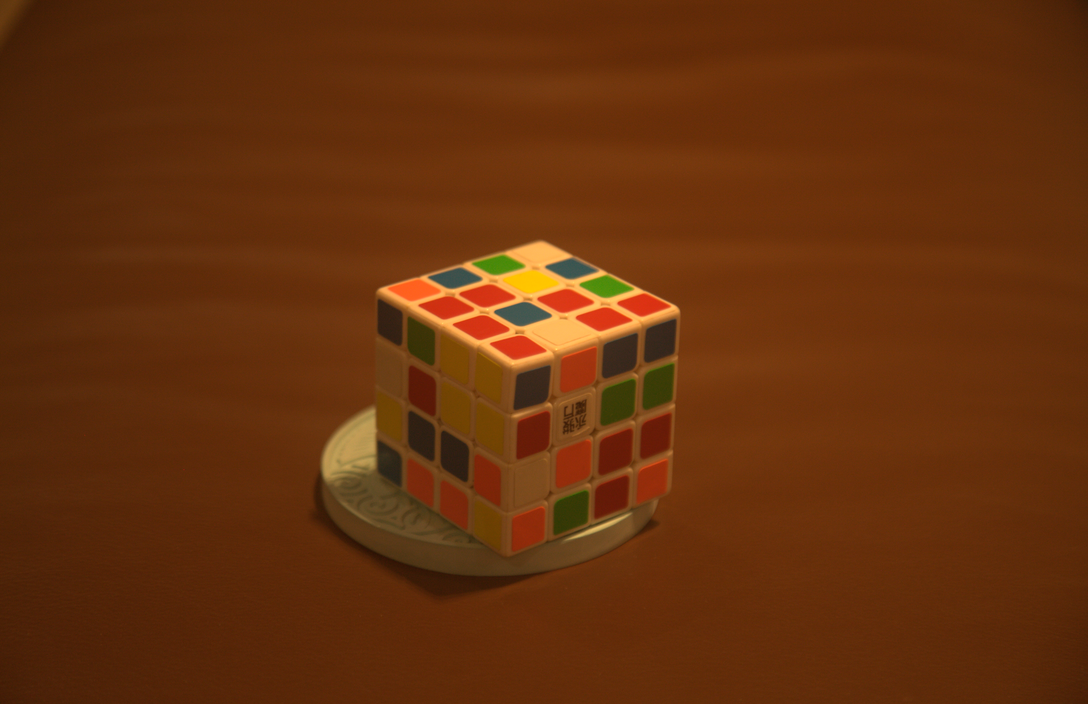
\includegraphics[width=\textwidth]{./implementation/experiment/out.png}
\end{center}
\end{subfigure}
\begin{subfigure}[b]{0.4\textwidth}
\caption{R colorspace}
\begin{center}
	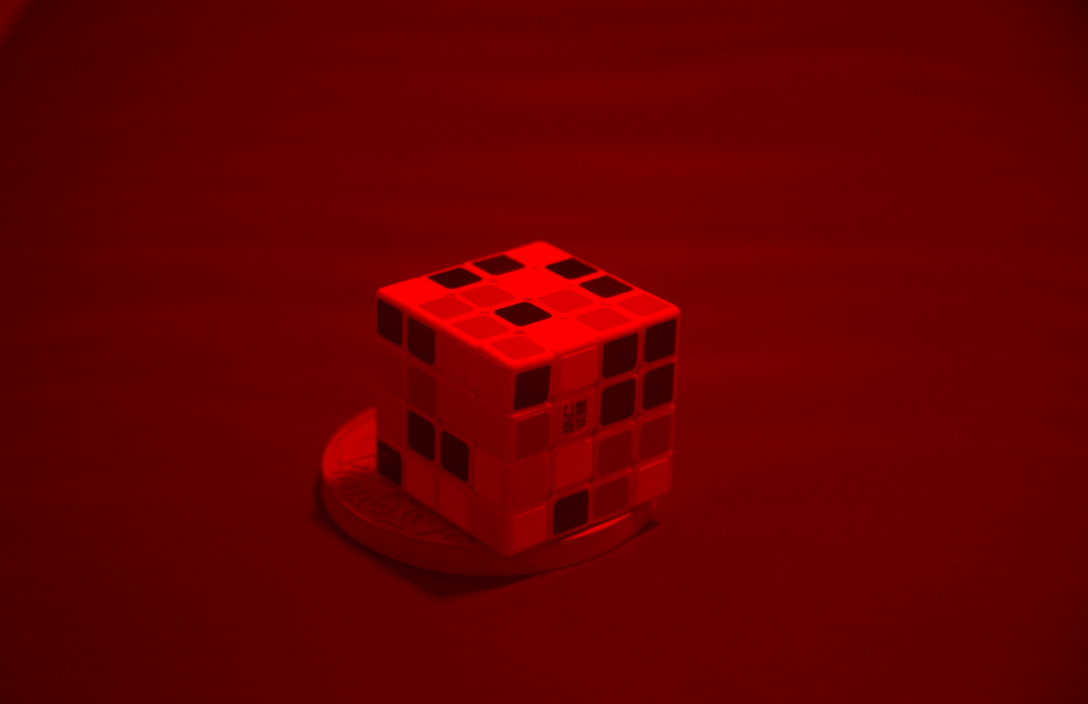
\includegraphics[width=\textwidth]{./implementation/experiment/red.png}
\end{center}
\end{subfigure}
\begin{subfigure}[b]{0.4\textwidth}
\begin{center}
	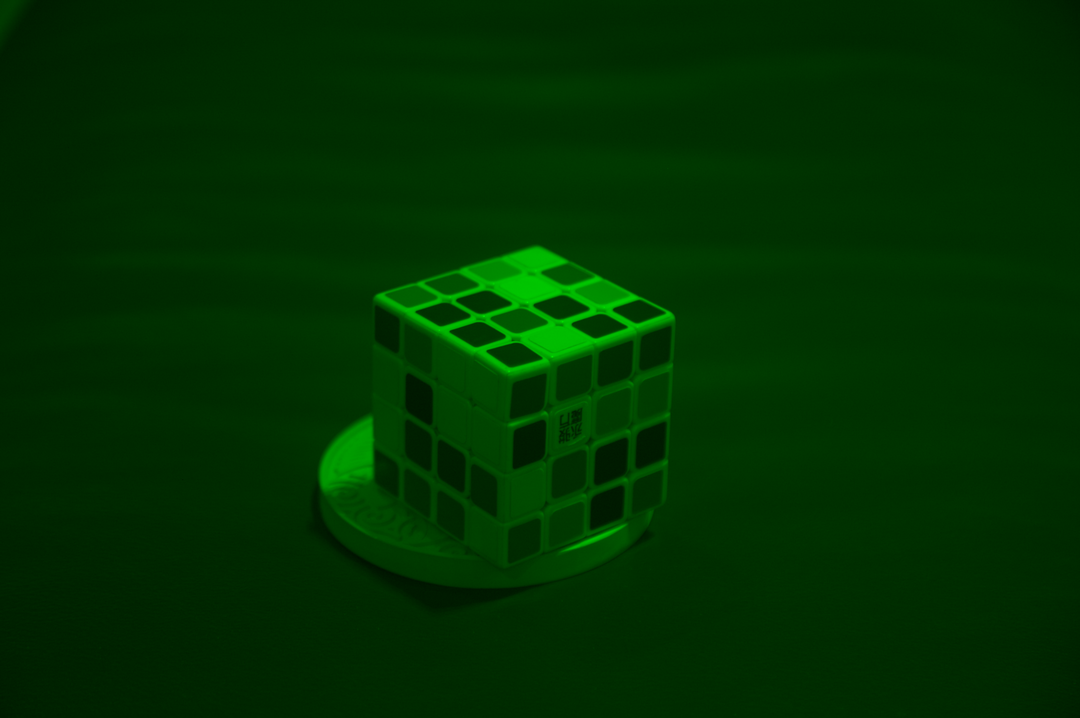
\includegraphics[width=\textwidth]{./implementation/experiment/green.png}
\end{center}
\caption{G colorspace}
\end{subfigure}
\begin{subfigure}[b]{0.4\textwidth}
\begin{center}
	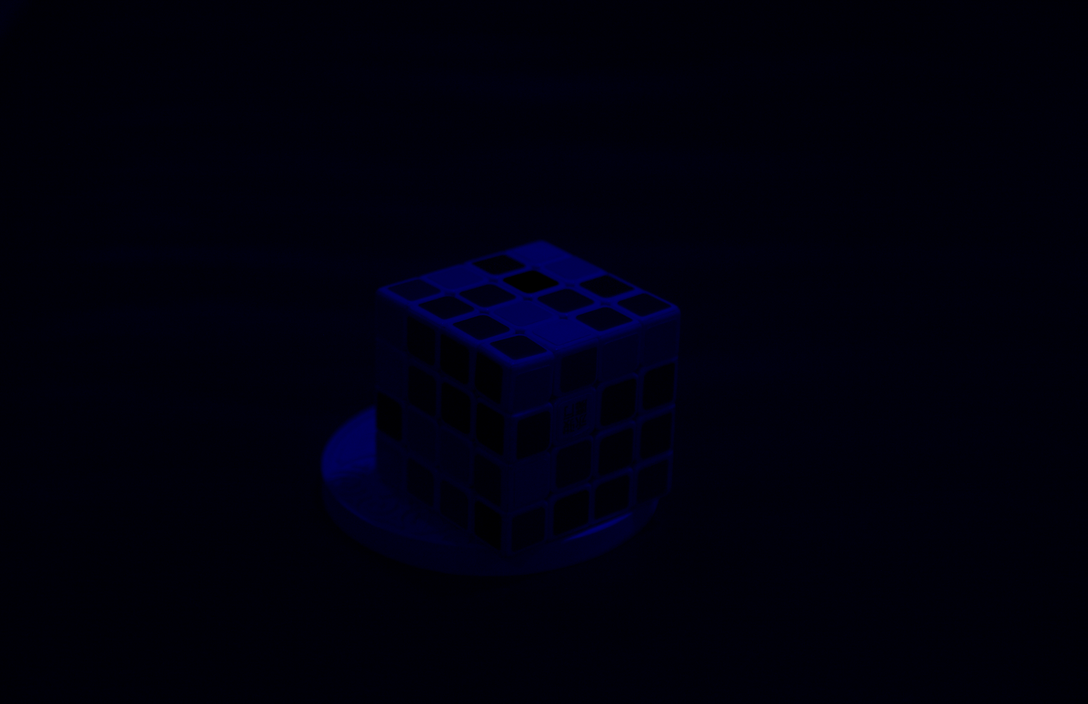
\includegraphics[width=\textwidth]{./implementation/experiment/blue.png}
\end{center}
\caption{B colorspace}
\end{subfigure}
\caption{\texttt{RGB} colorspace}
\label{fig:rgb}
\end{figure}

\begin{figure}[h!]
\centering
\begin{subfigure}[b]{0.4\textwidth}
\caption{Original Picture}
\begin{center}
	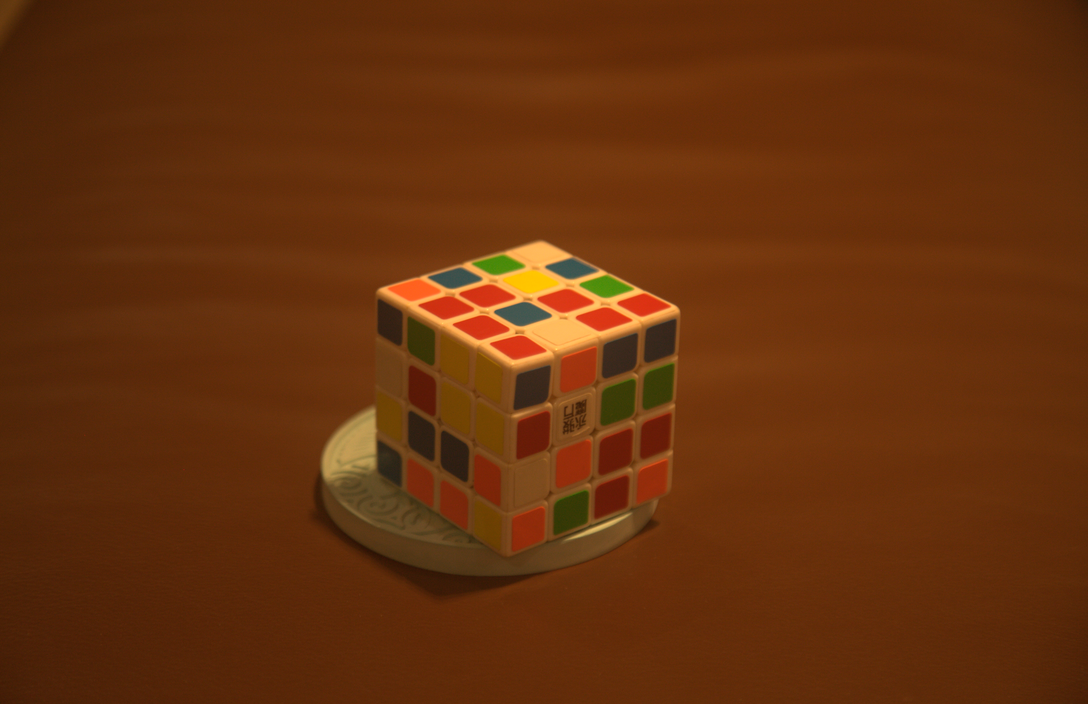
\includegraphics[width=\textwidth]{./implementation/experiment/out.png}
\end{center}
\end{subfigure}
\begin{subfigure}[b]{0.4\textwidth}
\caption{Luminance}
\begin{center}
	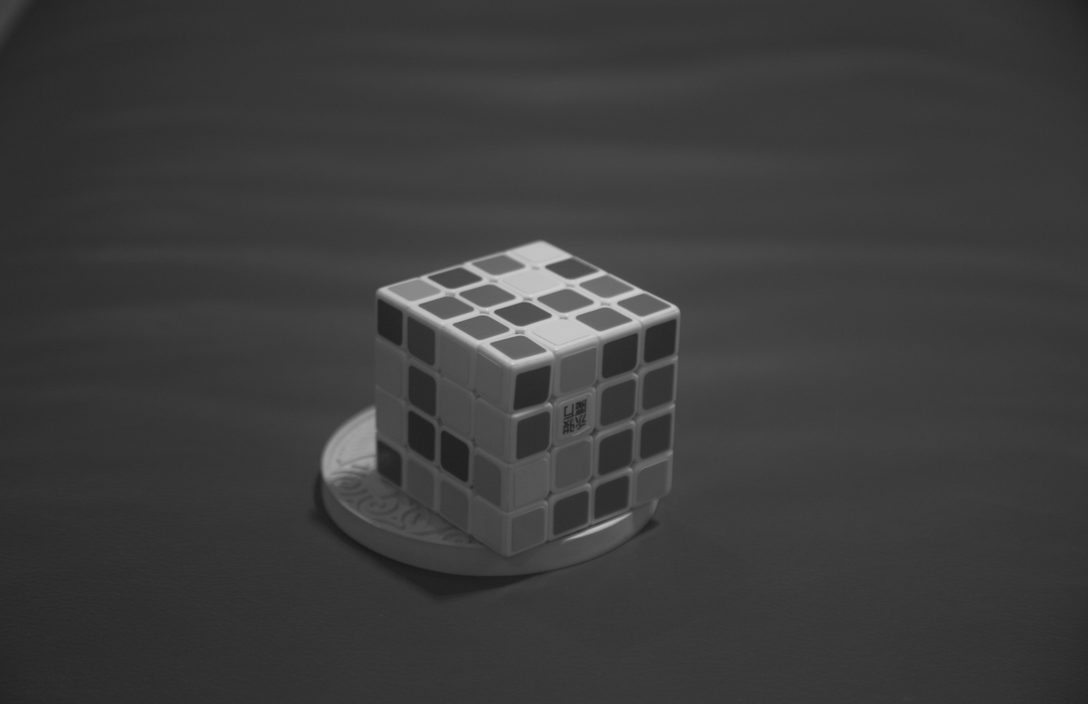
\includegraphics[width=\textwidth]{./implementation/experiment/Y.png}
\end{center}
\end{subfigure}
\begin{subfigure}[b]{0.4\textwidth}
\begin{center}
	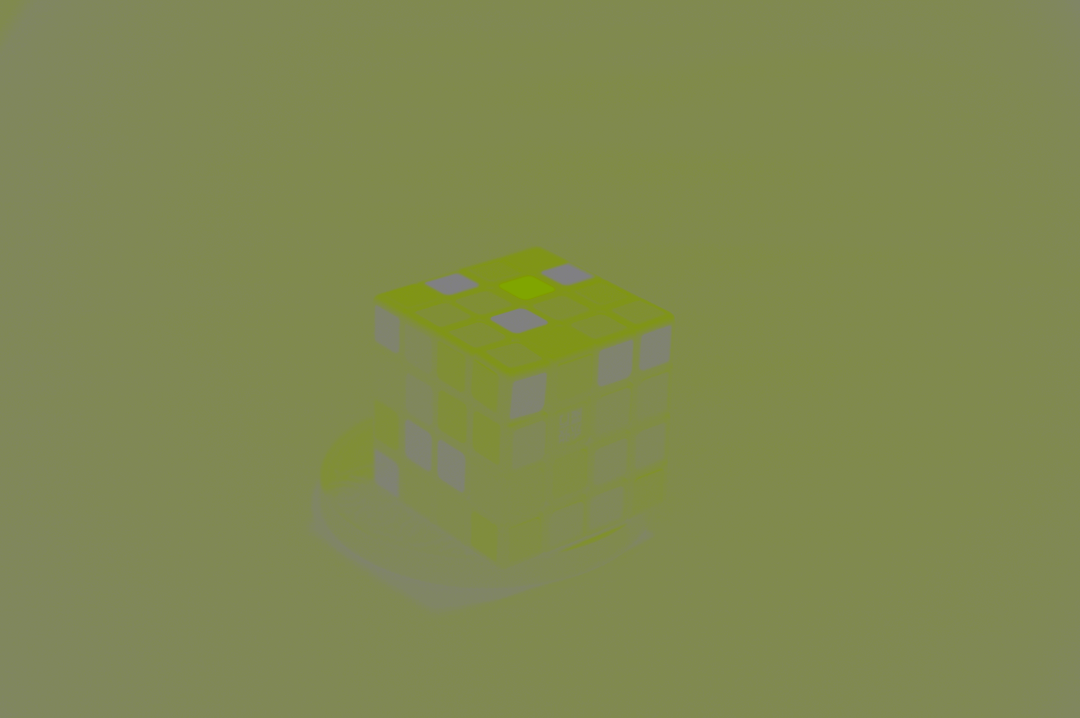
\includegraphics[width=\textwidth]{./implementation/experiment/Cb.png}
\end{center}
\caption{Chroma Blue}
\end{subfigure}
\begin{subfigure}[b]{0.4\textwidth}
\begin{center}
	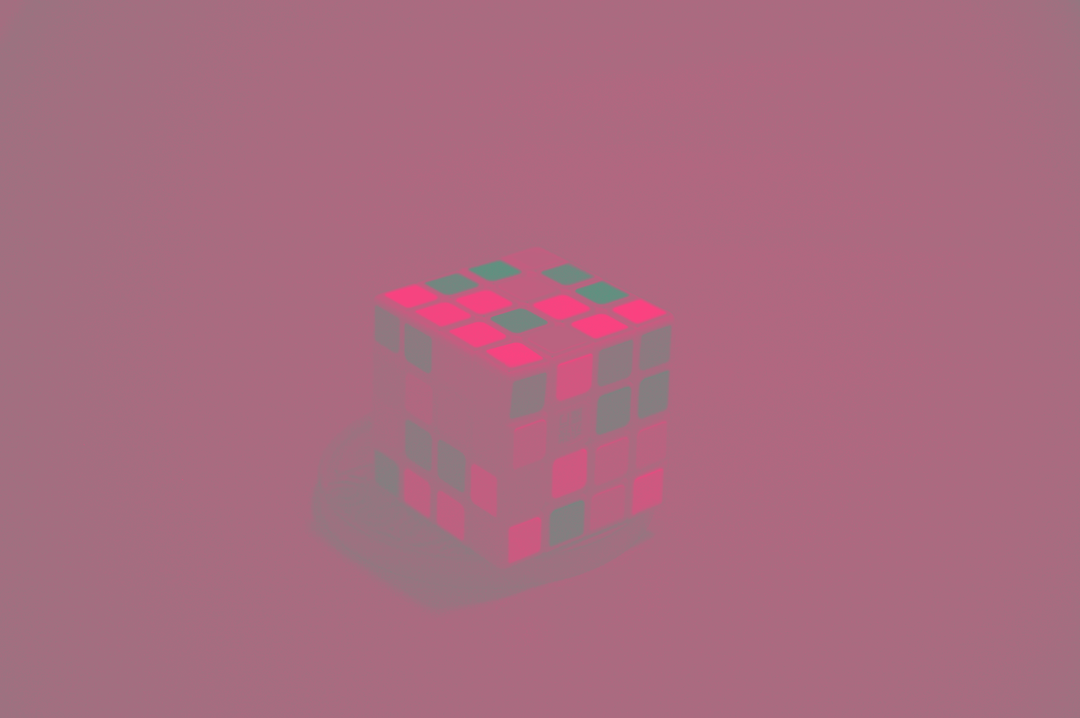
\includegraphics[width=\textwidth]{./implementation/experiment/Cr.png}
\end{center}
\caption{Chroma Red}
\end{subfigure}
\caption{\texttt{YCbCr} colorspace}
\label{fig:ycbcr}
\end{figure}

Figure~\ref{fig:rgb} shows the \texttt{RGB} colorspace.
Figure~\ref{fig:ycbcr} shows the same picture converted to \texttt{YCbCr} colorspace.

\subsubsection{Subsampling}
Humans are more sensitive to brightness that color.
Since the brightness (luminance) is stored as Y in YCbCr, and color (chroma) stored as Cb and Cr, we process them separately.
According to this statement, we can reduce the amount of details stored Cb and Cr, which would create minimal effects on the human eye.

We can perform this operation by only storing half (or any other arbitrary number) the amount of pixels.
When decompressing the image, the missing pixels would then be interpolated.
This could be done by averaging out the nearest two available pixels, or simply referring to the pixel or the left.

\begin{wrapfigure}{r}{0.4\textwidth}
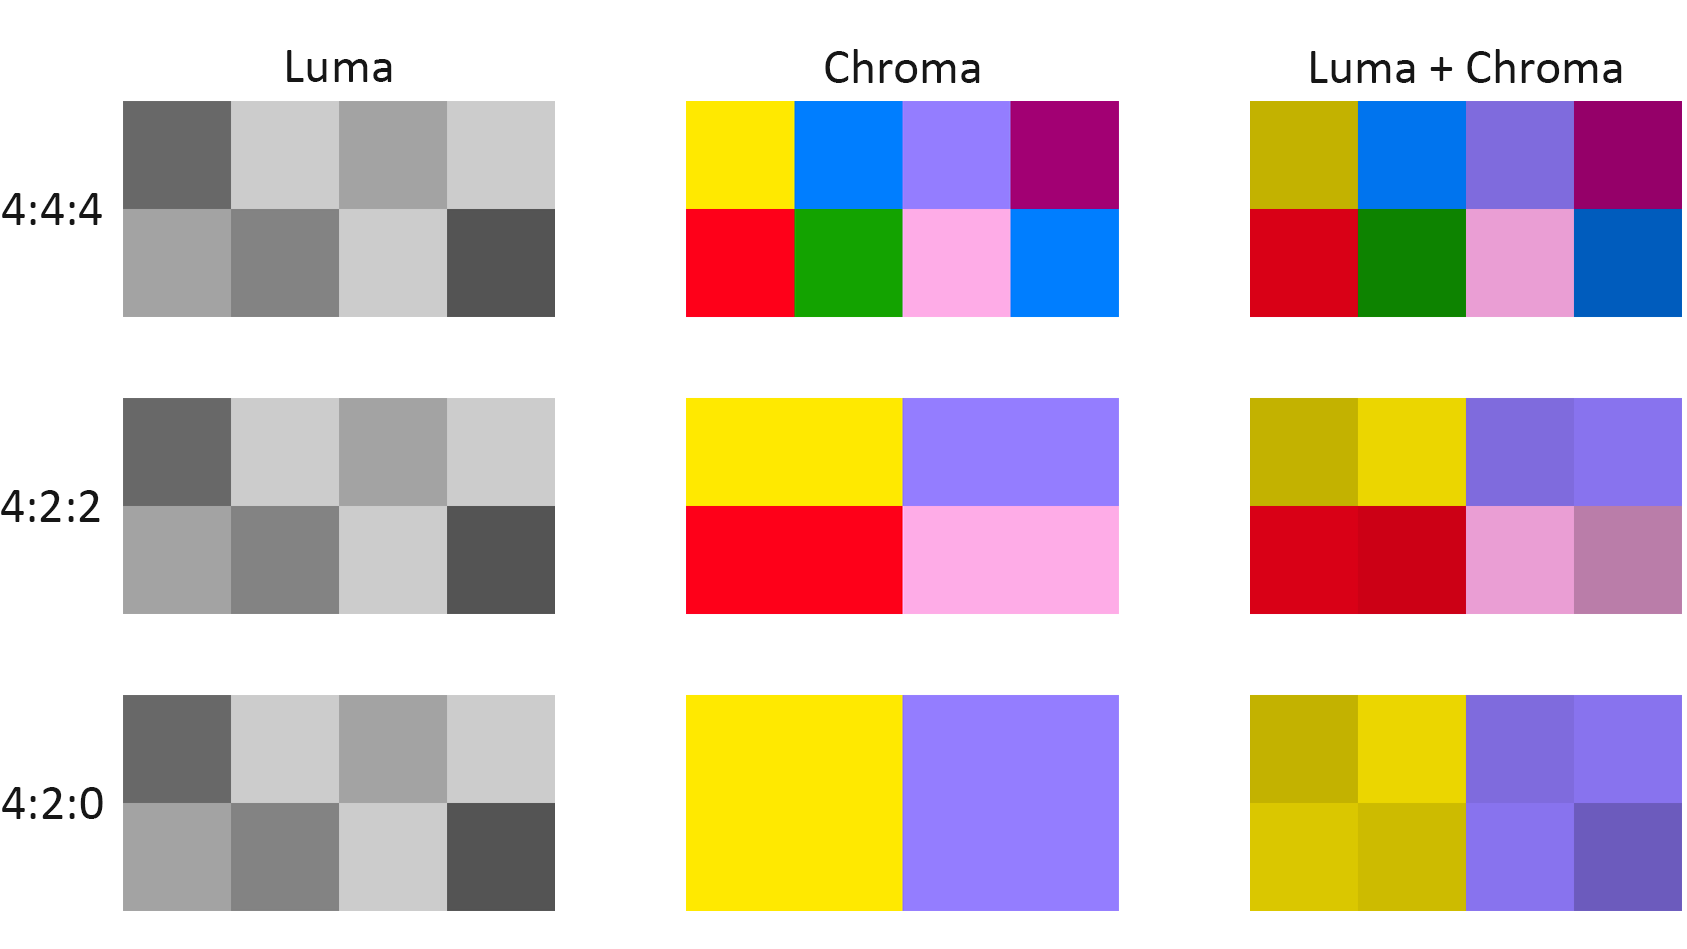
\includegraphics[width=\linewidth]{./figures/subsampling.png}
\caption{Chroma Subsampling illustrated}
\label{fig:subsampling}
\end{wrapfigure}

There are several common schemes for discarding pixels: \texttt{4:4:4}, \texttt{4:2:2}, and \texttt{4:2:0} (refer to figure~\ref{fig:subsampling}).
Note, only chroma pixels are discarded, as discarding luminance pixels makes a noticeable difference.
\texttt{4:4:4} discards no pixels, essentially no sub sampling.
\texttt{4:2:2} discards every second column, discarding half the pixels.
\texttt{4:2:0} discards every second column and every second row, discarding $\frac{3}{4}$ of the pixels.
A less common \texttt{4:1:1} keeps only every fourth column, discarding $\frac{3}{4}$ of the pixels (but vertically).

The code used for chroma subsampling is listed below:
\begin{lstlisting}{language=python}
def comp422(inp):
    """4:2:2 chroma subsampling"""
    Y, Cr, Cb = cv2.split(inp)
    x, y = Y.shape
    comp_Cb = np.empty([x, y//2], dtype=np.uint8)
    comp_Cr = np.empty([x, y//2], dtype=np.uint8)

    for i in range(comp_Cb.shape[0]):
        for j in range(comp_Cb.shape[1]):
            comp_Cb[i][j] = Cb[i][j*2]

    for i in range(comp_Cr.shape[0]):
        for j in range(comp_Cr.shape[1]):
            comp_Cr[i][j] = Cr[i][j*2]

    return Y, comp_Cb, comp_Cr


def comp411(inp):
    """4:1:1 chroma subsampling"""
    Y, Cr, Cb = cv2.split(inp)
    x, y = Y.shape
    comp_Cb = np.empty([x, y//4], dtype=np.uint8)
    comp_Cr = np.empty([x, y//4], dtype=np.uint8)

    for i in range(comp_Cb.shape[0]):
        for j in range(comp_Cb.shape[1]):
            comp_Cb[i][j] = Cb[i][j*4]

    for i in range(comp_Cr.shape[0]):
        for j in range(comp_Cr.shape[1]):
            comp_Cr[i][j] = Cr[i][j*4]

    return Y, comp_Cb, comp_Cr


def comp420(inp):
    """4:2:0 chroma subsampling"""
    Y, Cr, Cb = cv2.split(inp)
    x, y = Y.shape
    comp_Cb = np.empty([x//2, y//2], dtype=np.uint8)
    comp_Cr = np.empty([x//2, y//2], dtype=np.uint8)

    for i in range(comp_Cb.shape[0]):
        for j in range(comp_Cb.shape[1]):
            comp_Cb[i][j] = Cb[i*2][j*2]

    for i in range(comp_Cr.shape[0]):
        for j in range(comp_Cr.shape[1]):
            comp_Cr[i][j] = Cr[i*2][j*2]

    return Y, comp_Cb, comp_Cr
\end{lstlisting}

\texttt{np.empty} creates two empty arrays \texttt{comp\_Cb} and \texttt{comp\_Cr}.
The array length depends on the type of chroma subsampling (\texttt{[x, y//2]}).
\texttt{dtype=np.uint8} defines the array to store an image.
The \texttt{for} loop then iterates through the original chroma arrays, and selectively\footnote{\texttt{[i*2][j*2]} in this case skip 1 pixel horizontally and vertically} copies the pixels over.

\begin{figure}[h!]
\centering
\begin{subfigure}[b]{0.4\textwidth}
\caption{\texttt{4:4:4}}
\begin{center}
	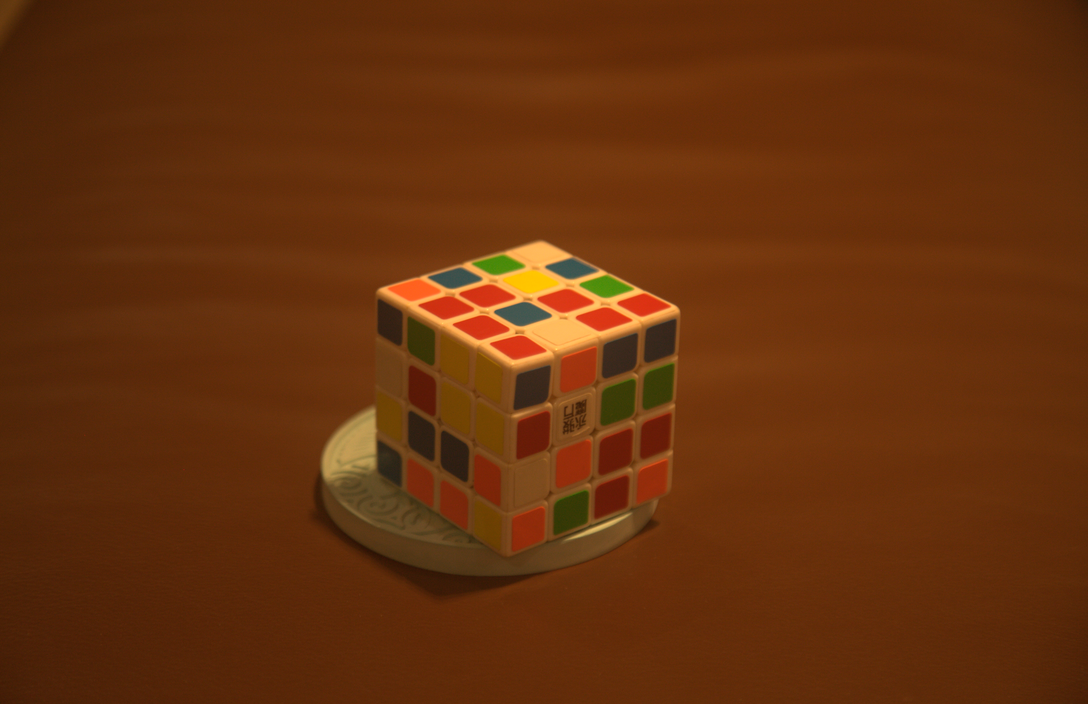
\includegraphics[width=\textwidth]{./implementation/experiment/out.png}
\end{center}
\end{subfigure}
\begin{subfigure}[b]{0.4\textwidth}
\caption{\texttt{4:2:2}}
\begin{center}
	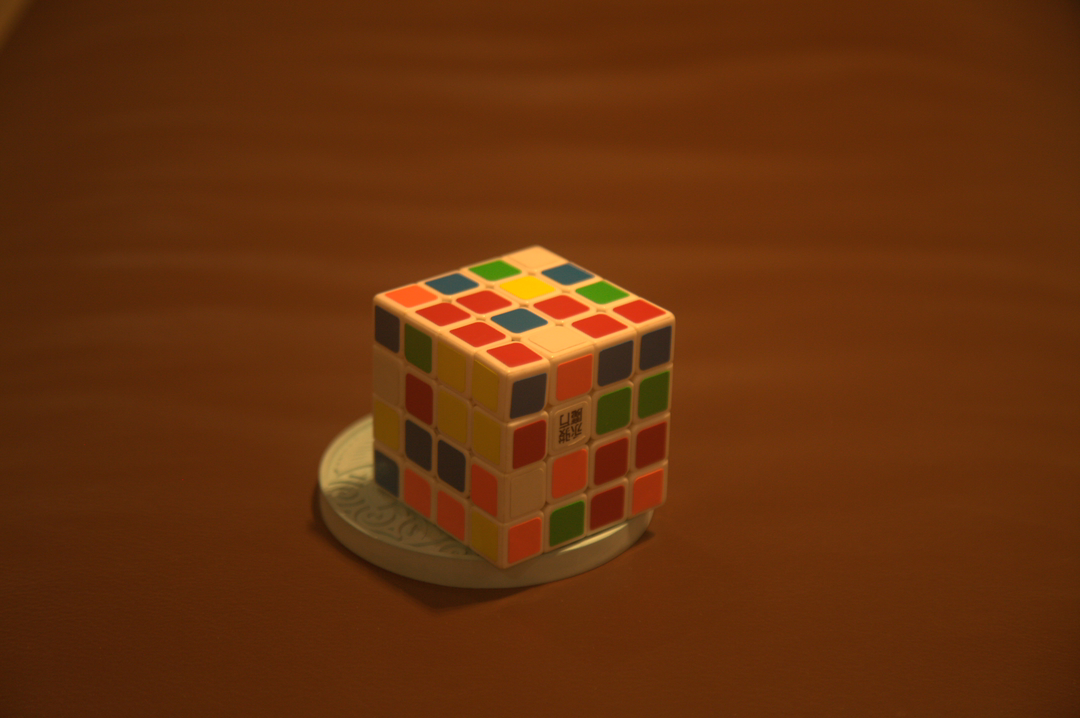
\includegraphics[width=\textwidth]{./implementation/experiment/422.png}
\end{center}
\end{subfigure}
\begin{subfigure}[b]{0.4\textwidth}
\begin{center}
	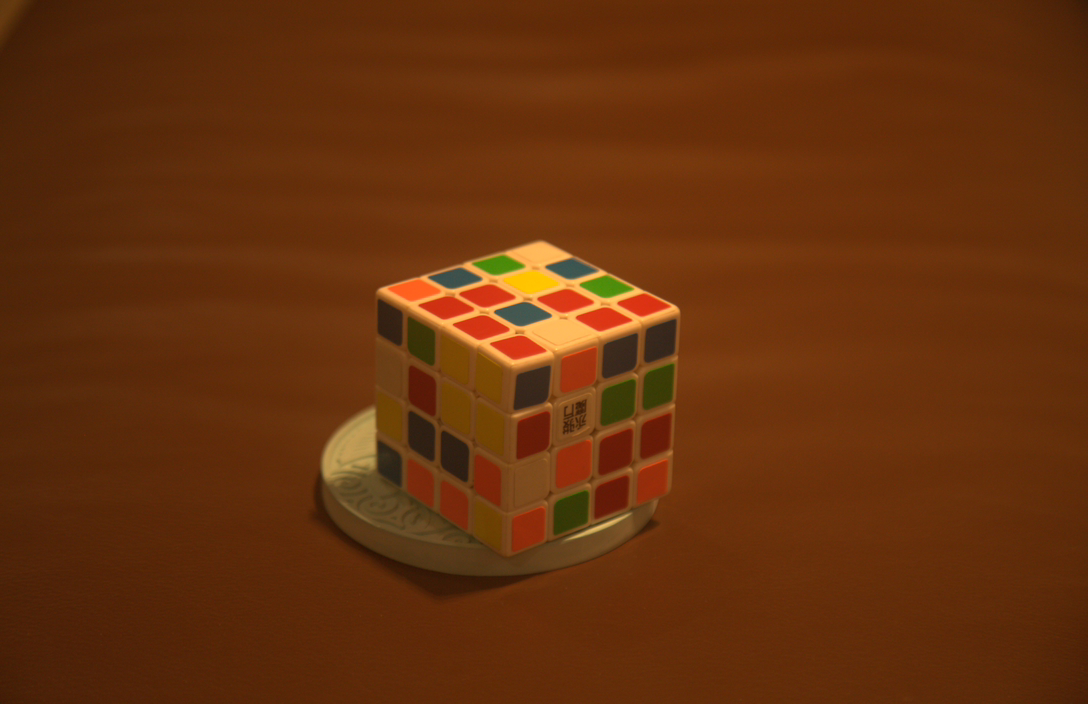
\includegraphics[width=\textwidth]{./implementation/experiment/420.png}
\end{center}
\caption{\texttt{4:2:0}}
\end{subfigure}
\begin{subfigure}[b]{0.4\textwidth}
\begin{center}
	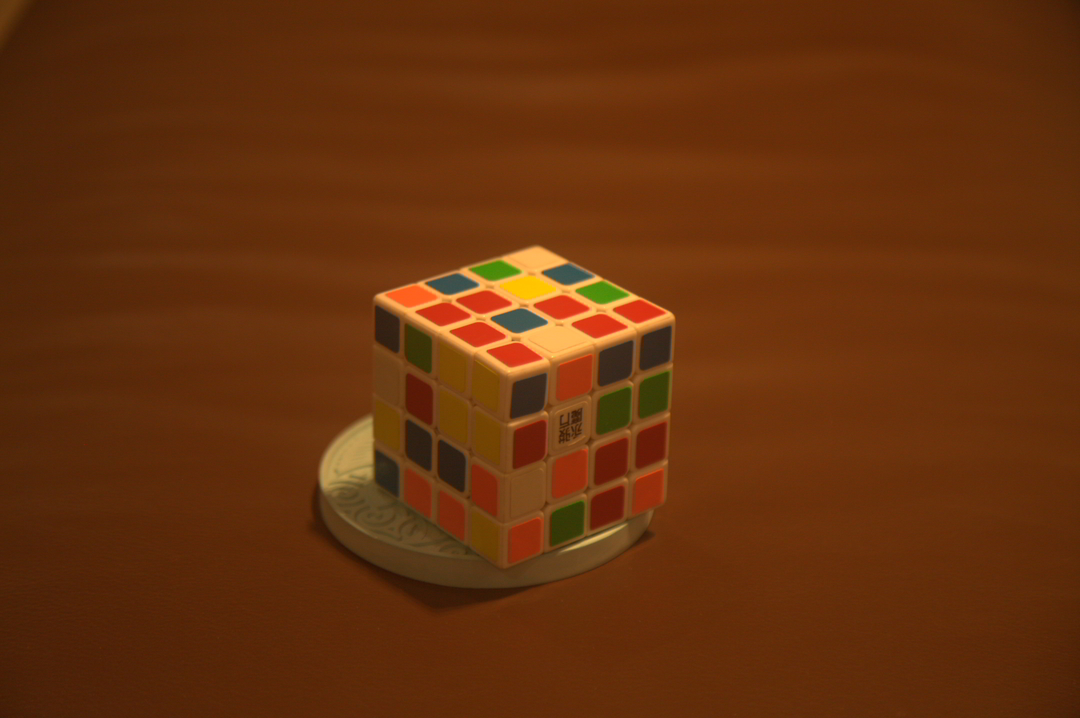
\includegraphics[width=\textwidth]{./implementation/experiment/411.png}
\end{center}
\caption{\texttt{4:1:1}}
\end{subfigure}
\caption{Different types of chroma subsampling}
\label{fig:chroma}
\end{figure}

Figure~\red{fig:chroma} shows the end result of chroma subsampling.
The even after discarding $75\%$ of the color data (\texttt{4:2:0}), the human cannot easily perceive the difference in image quality.
However, when zoomed in, the details are somewhat noticeable.
Especially on sharp edges and quick changes in color.

\subsection{Discrete Cosine Transform}\label{dct}
Discrete Cosine Transform (DCT) separates an image into frequency components.
DCT is a subset of Fourier Transformation~\autocite{dctYT}, which takes a time based function and transforms it into the frequency and amplitude components.
This is performed by first splitting an image into small 8 by 8 pixel chunks, then performing the algorithm.
Although the DCT used on imaged are 2 dimensions, we can explain the concept from a 1 dimension perspective first.

\begin{figure}[h]
\centering
\begin{subfigure}[b]{0.45\textwidth}
	\centering
	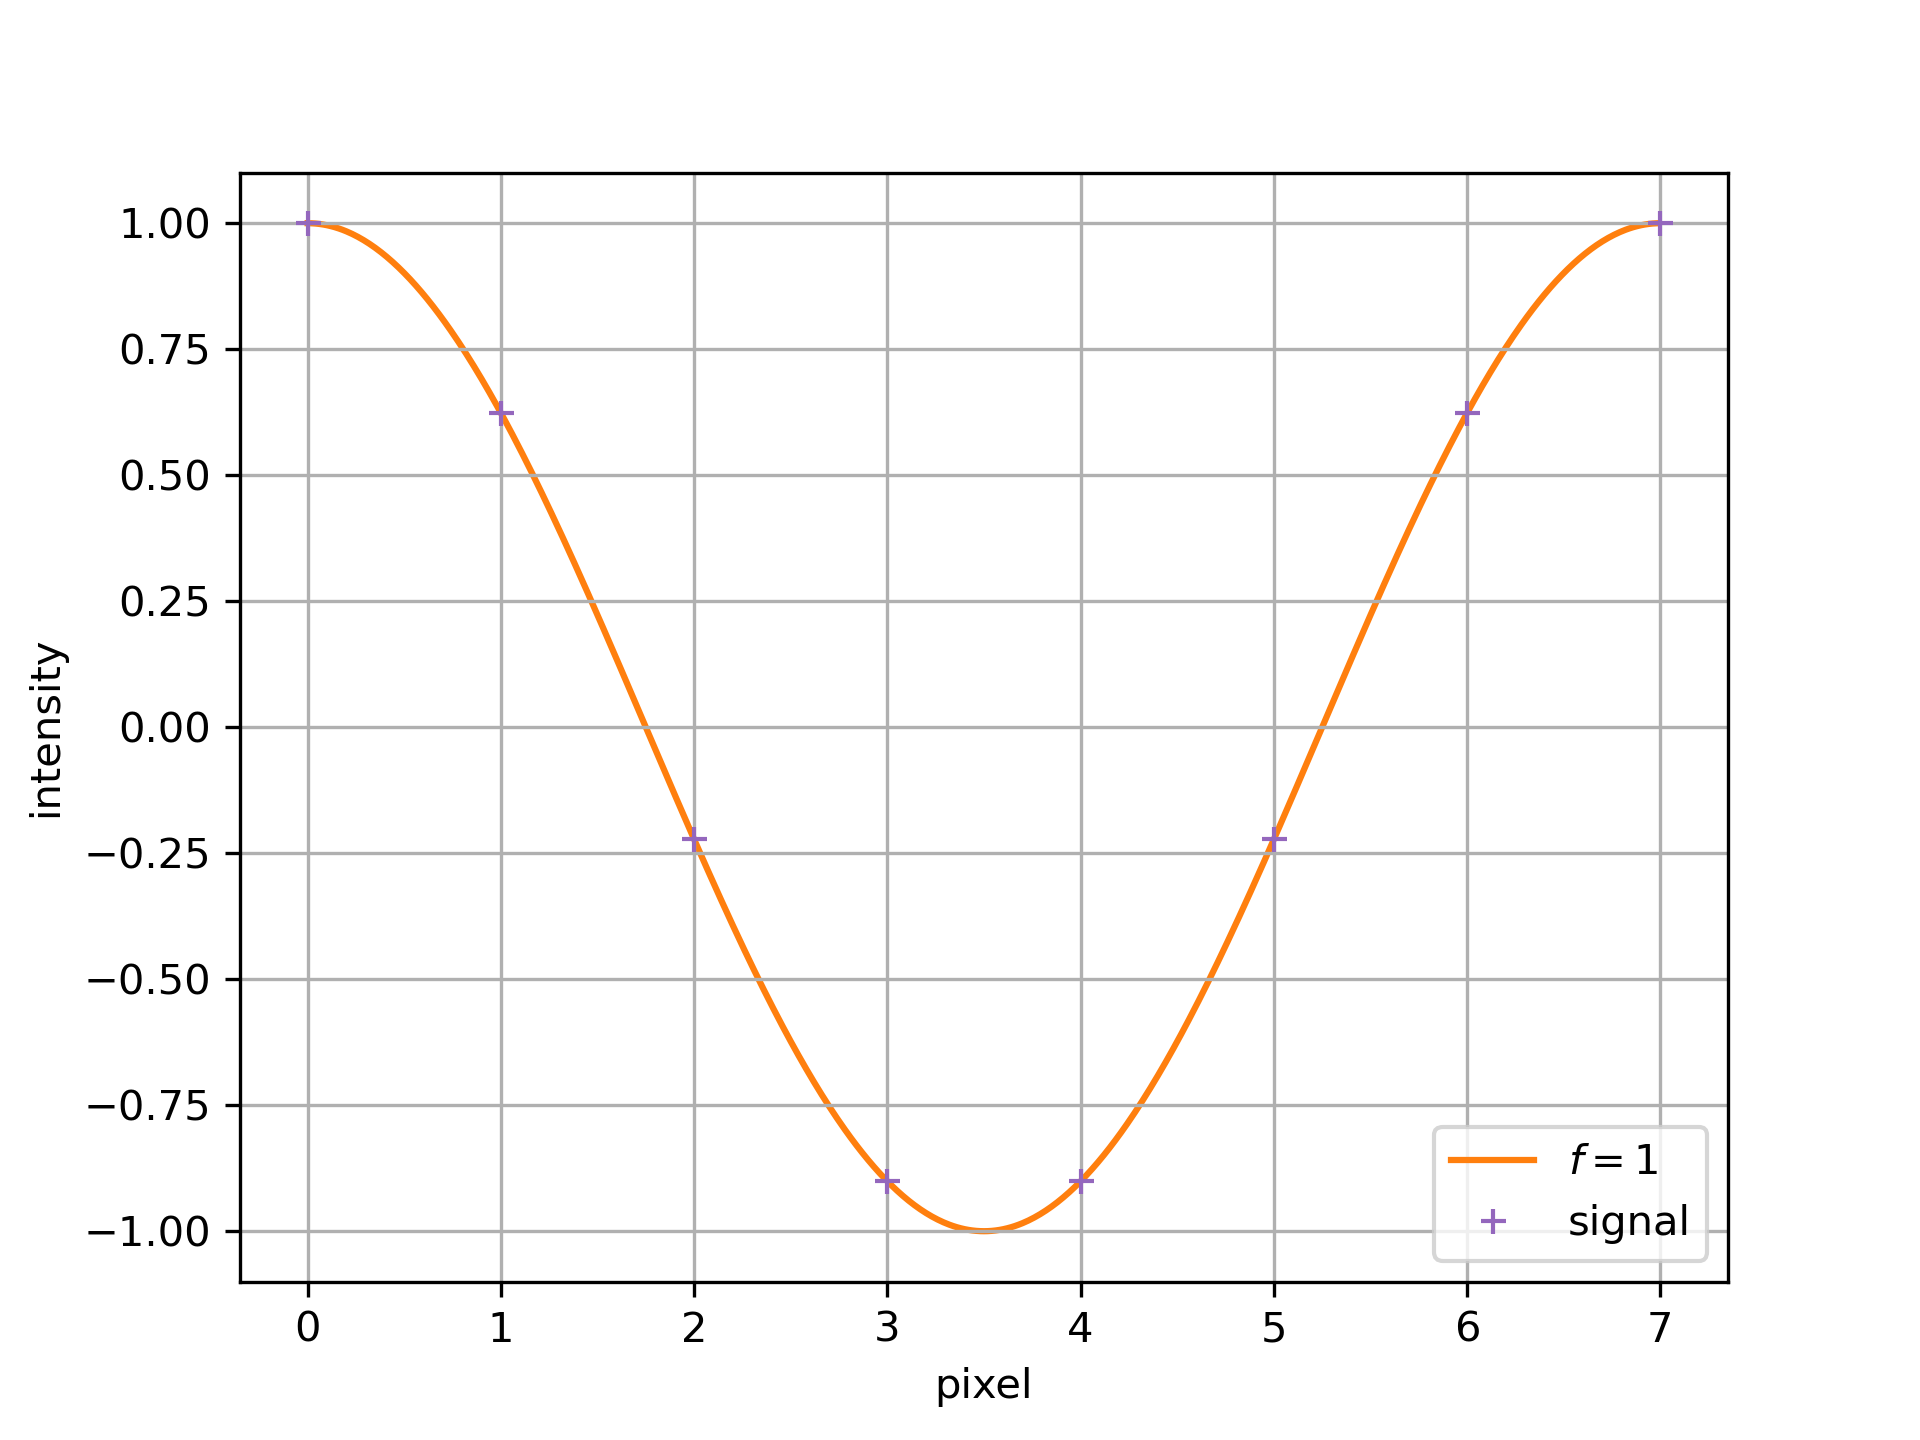
\includegraphics[width=\textwidth]{./figures/dct/cos1}
	\caption{$f = 1$}
	\label{fig:cos1}
\end{subfigure}
\begin{subfigure}[b]{0.45\textwidth}
	\centering
	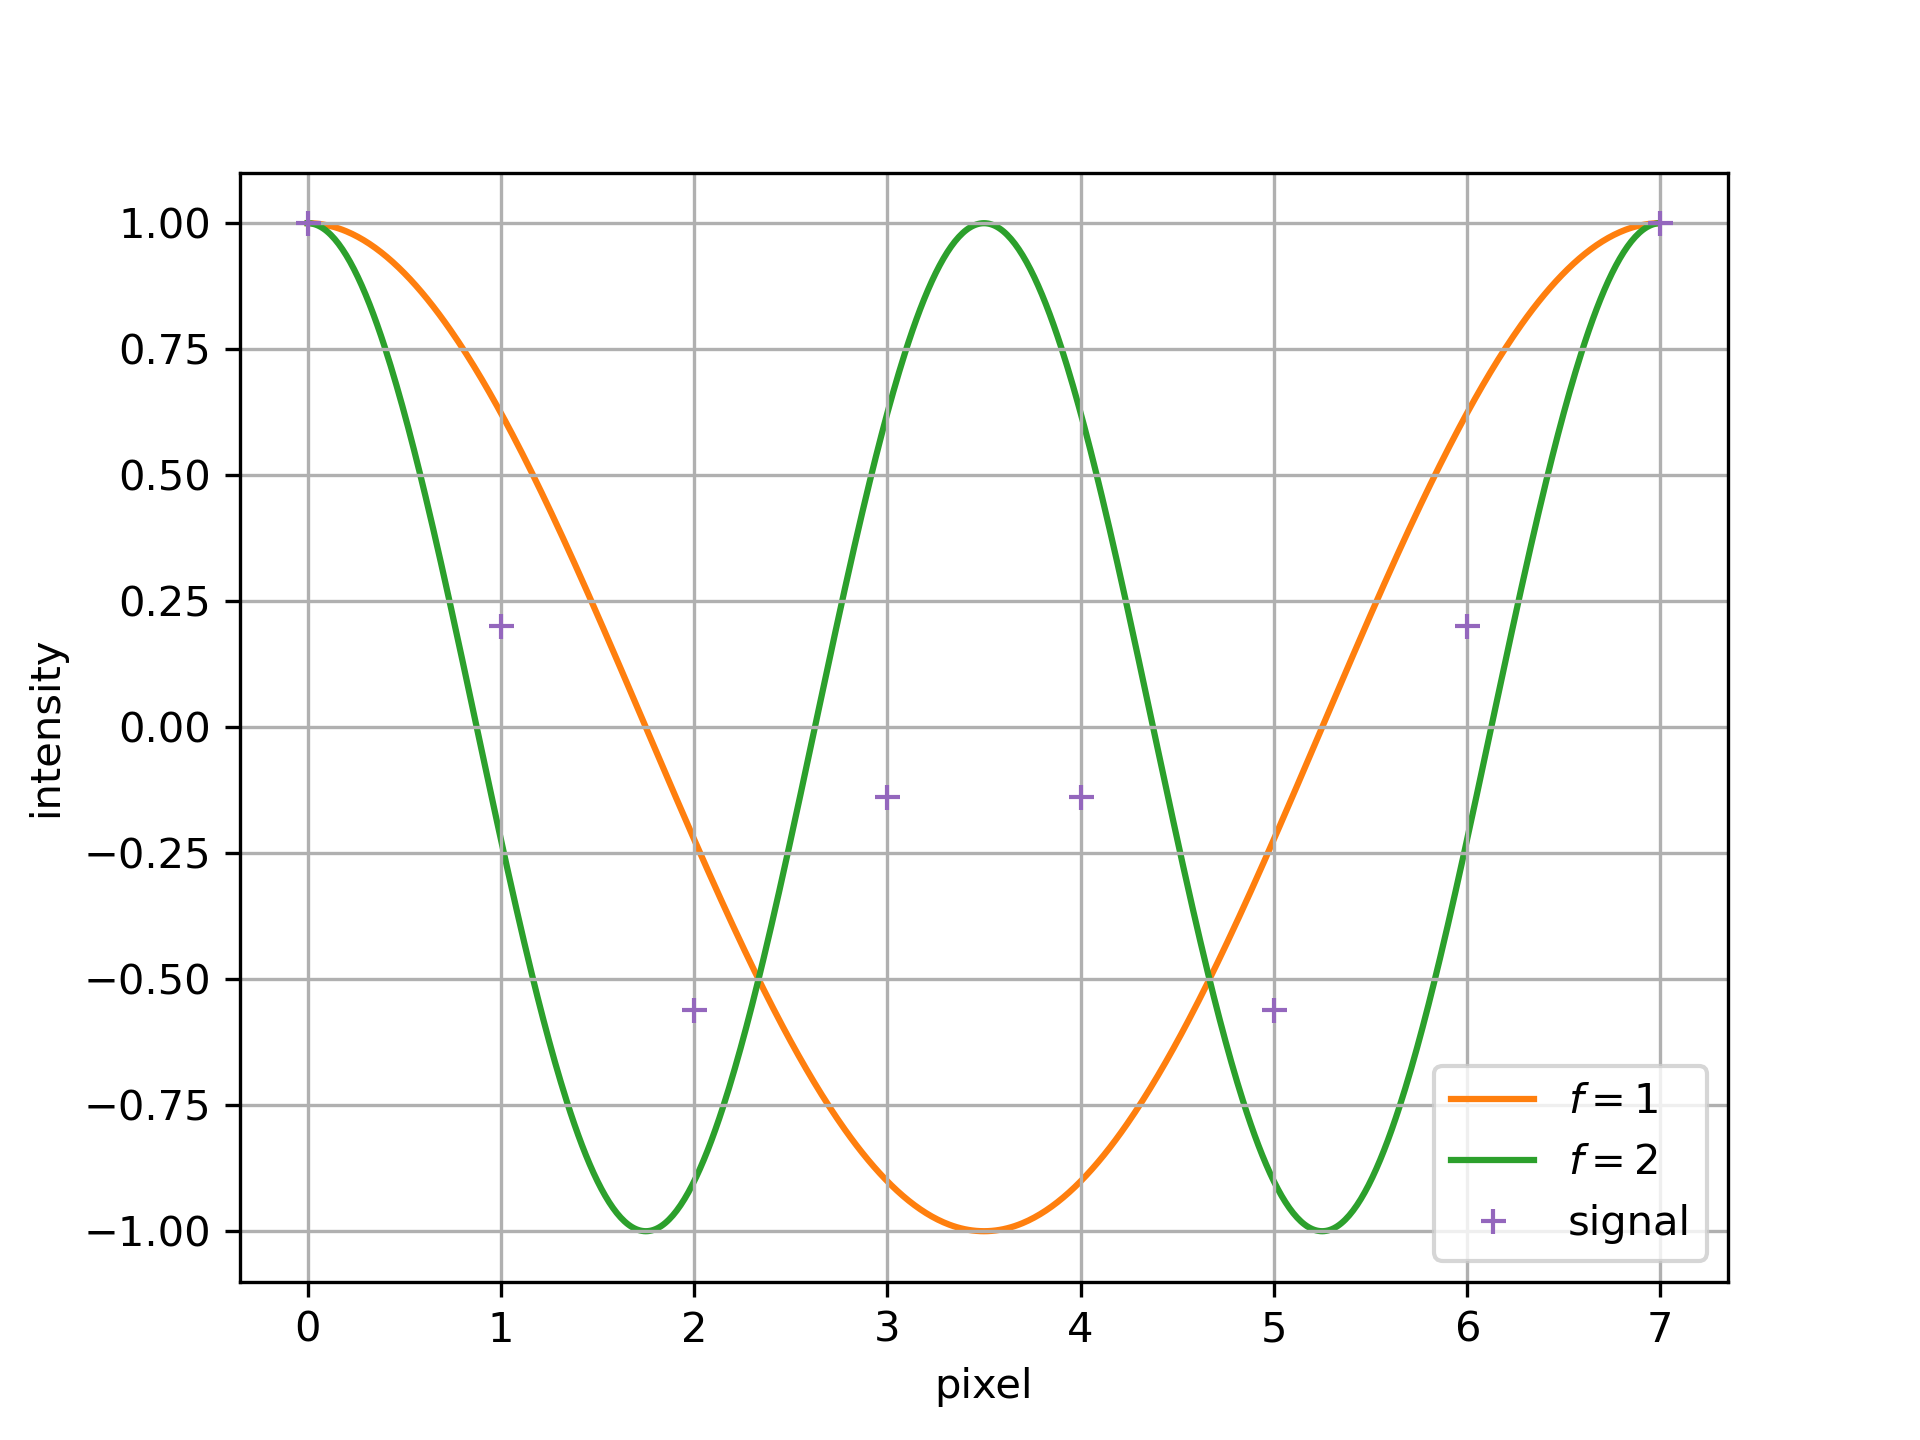
\includegraphics[width=\textwidth]{./figures/dct/cos2}
	\caption{$f=1\, + \, f = 2$}
	\label{fig:cos2}
\end{subfigure}
\begin{subfigure}[b]{0.45\textwidth}
	\centering
	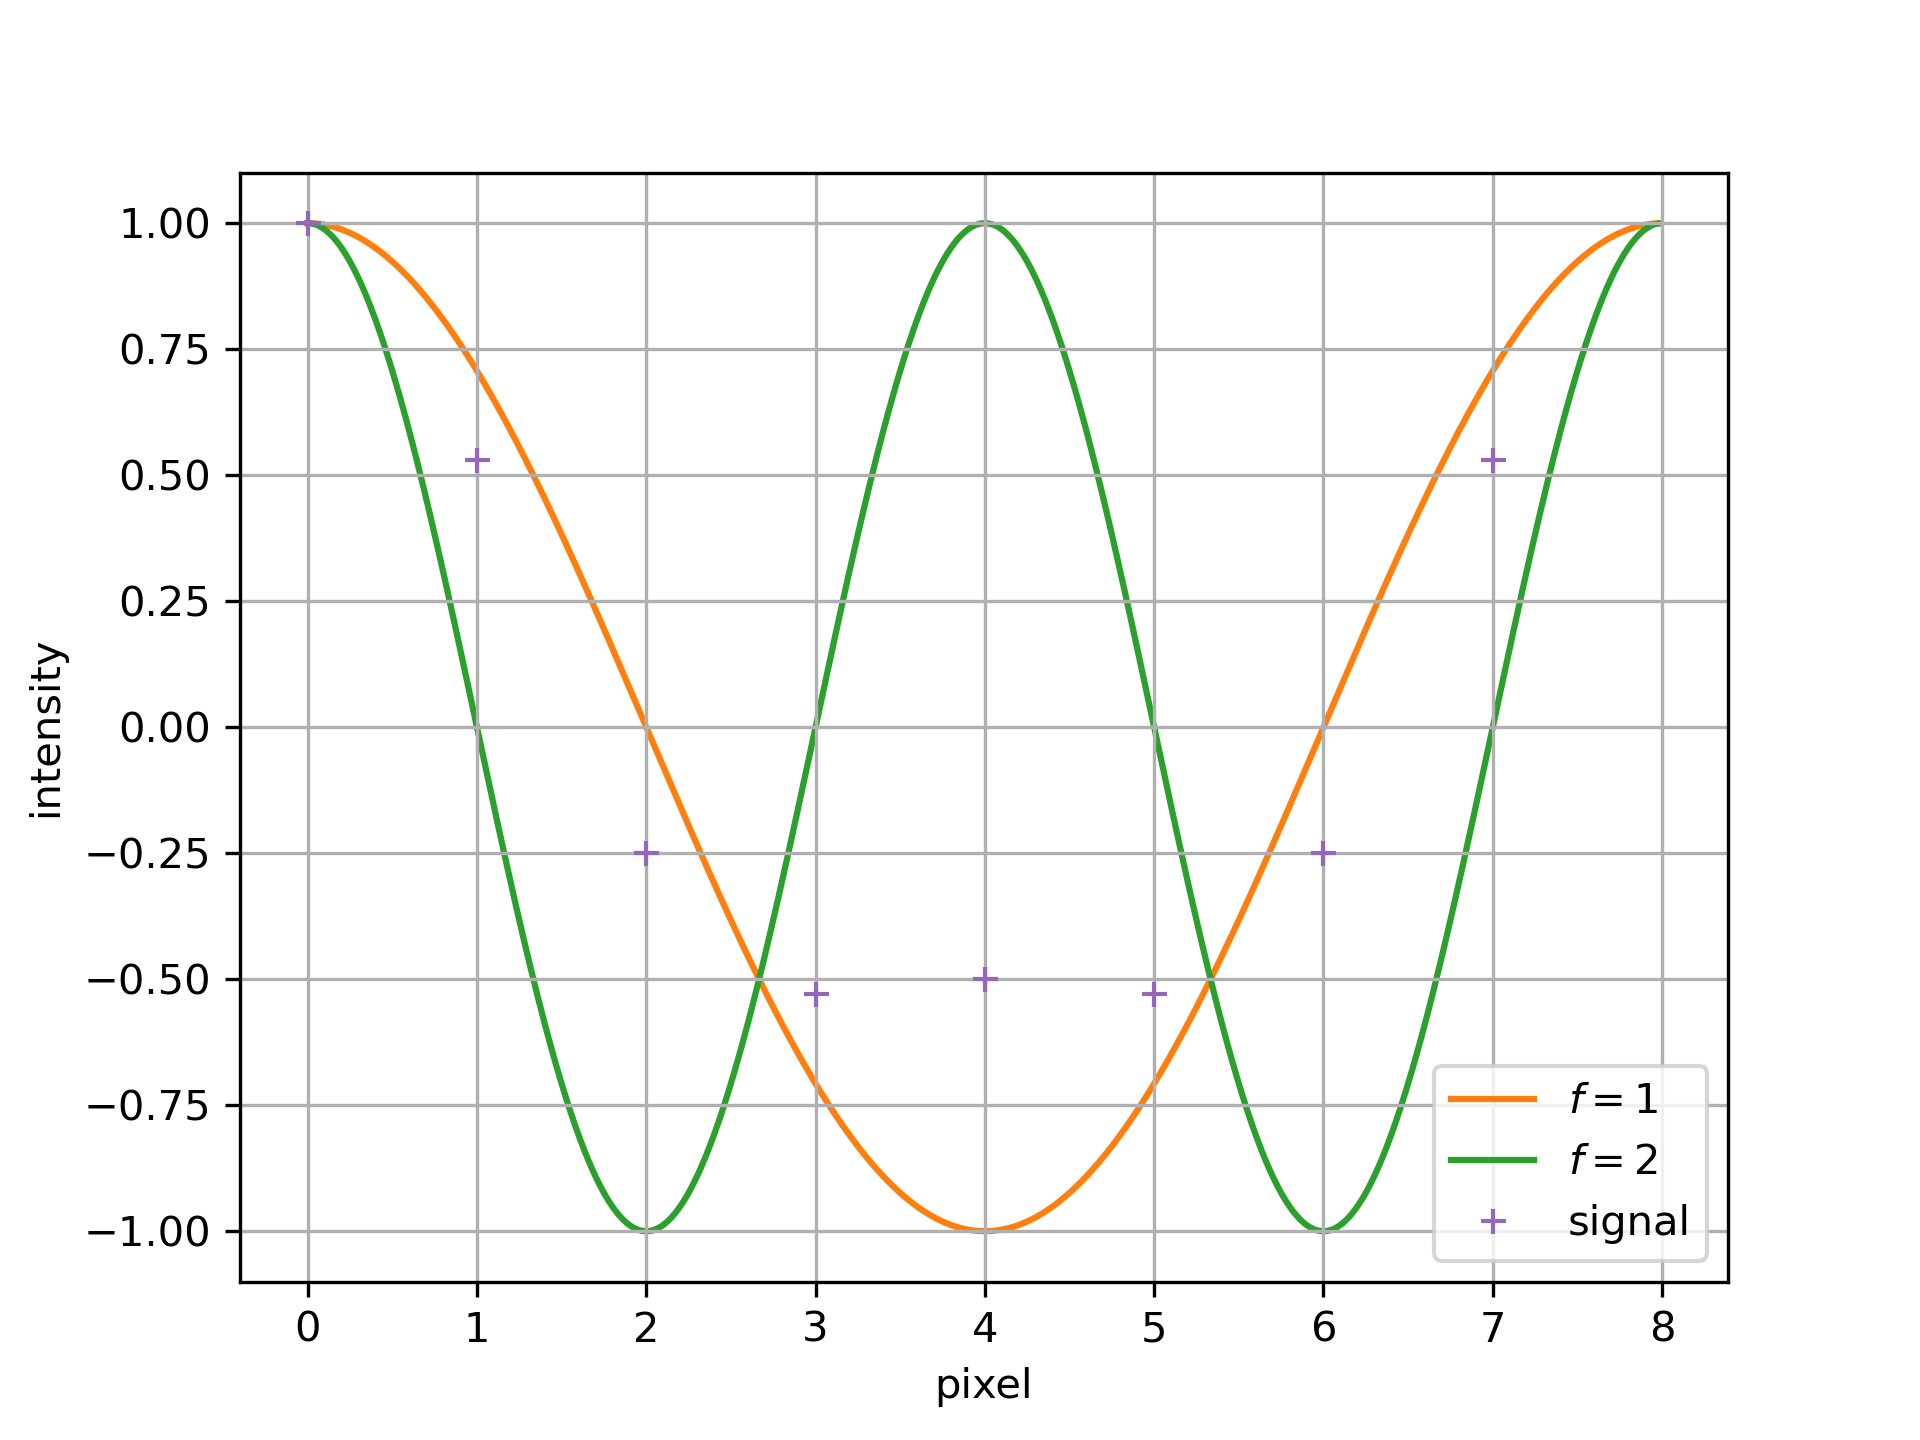
\includegraphics[width=\textwidth]{./figures/dct/cos3}
	\caption{Weighted cosine curves}
	\label{fig:cos3}
\end{subfigure}
\caption{Cosine curves with varying frequency}
\end{figure}

Lets take a single row of 8 pixels, and plot them on a graph with pixels on the x axis and intensity on the y axis.
The resulted data points forms a signal.
If we were to recreate the curve mathematically, we can plot a curve through the data points.
DCT reconstructs the signal by stacking differently weighted cosine curves of different frequency and amplitude.

For example, figure~\ref{fig:cos1} shows a cosine curve with a period of 8 pixels.
Lets say this curve has a frequency of 1 unit.
The purple coordinates represents the resultant signal.

If we add an additional cosine curve with a frequency of 2 units, the signal will be changed.
In this case, the signal is the average of both curves.

If we change to weighting of the average, we can change the signal.
In this case, the cosine curve with a frequency of 1 unit is weighed 3 times as much as the other cosine curve.

DCT\footnote{More specifically DCT-II, used by JIFF compression} propose that we can represent any signal by adding 8 weighted cosine curves of increasing frequency.
The resulted signal is modeled by this mathematical equation.
The exact mathematics of DCT is too advance for the scope of this paper, implementation of DCT will be done through code.
\begin{equation}
	X_k = \sum_{n=0}^{N-1} x_n \cos \left [ \frac{\pi}{N} \left ( n + \frac{1}{2} \right ) \right ] \qquad k = 0, \dots , N - 1
\end{equation}

% explain why with notation table

\texttt{Continue with an example here (use random number and find the frequency)}

The example showed 1 dimension DCT, 2 dimension DCT is used on photos.
Similar to decomposing a signal into many stacking cosine waves, 2D DCT decompose an 8 by 8 image into a stack of 8 by 8 grids.
These grids are formed by 2D cosine waves, each with increasing frequency.
2D DCT proposes that an 8 by 8 image can be taken apart into 64 different cosine grids.
The results generated by this operation is called the DCT coefficients.

\subsection{Quantization}\label{quantize}
The beauty of DCT lies in that most of the image can be recreated by the lower frequency cosine blocks~\autocite{jpgYT}.
This is exploiting the second flaw in the human eye, reduced ability to see high frequency content.
Through this logical, we can theoretically create an importance value for each cosine grid (from DCT).
Using this importance value, we can throw away the less important data, while keeping the more important data.
This process is called quantization.

\begin{figure}[h]
\centering
\begin{equation}
	\begin{bmatrix}
		8  & 6  & 6  & 8  & 12 & 14 & 16 & 17 \\
		6  & 6  & 6  & 8  & 10 & 13 & 12 & 15 \\
		6  & 6  & 7  & 8  & 13 & 14 & 18 & 24 \\
		8  & 8  & 8  & 14 & 13 & 19 & 24 & 35 \\
		12 & 10 & 13 & 13 & 20 & 26 & 34 & 39 \\
		14 & 13 & 14 & 19 & 26 & 34 & 39 & 39 \\
		16 & 12 & 18 & 24 & 34 & 39 & 39 & 39 \\
		17 & 15 & 24 & 35 & 39 & 39 & 39 & 39
	\end{bmatrix}
\end{equation}
\label{fig:quantization}
\caption{Luminance quantization table from Photoshop Save To Web 050~\autocite{quantization}}
\end{figure}

This is done mathematically by dividing the DCT coefficients by a quantization table.
Each element in the DCT coefficients is divided by their responding quantization table, the resulted value rounded and stored as the quantized data matrix.
The process of rounding quantized data is removing information depending on the importance of each frequency.
Notice how in figure~\ref{fig:quantization}, the element in the quantization table increases as we move to the bottom right corner.
The higher the quantization factor, the lower the importance of that specific frequency block.

We can imagine the rounding process as a process of finding factors.
By dividing the DCT coefficients with the quantization coefficients, we are forcefully factoring the DCT coefficients by the quantization coefficients.
The smaller the quantization coefficient, the more accurate we can factor the DCT coefficients.
By tuning the quantization coefficients, we can control how much data about a specific frequency to throw out.

\subsection{Run Length Encoding}
After quantization, the resulted matrix is compressed into a string.
Due to the increased amount of quantization the further south east down the matrix, the quantized matrix often have a lot of similar values towards the south east side.
In order to take advantage of this repetition, a pointer will traverse the matrix in a zig zag manner, compacting it into a string.

\begin{wrapfigure}{r}{0.3\textwidth}
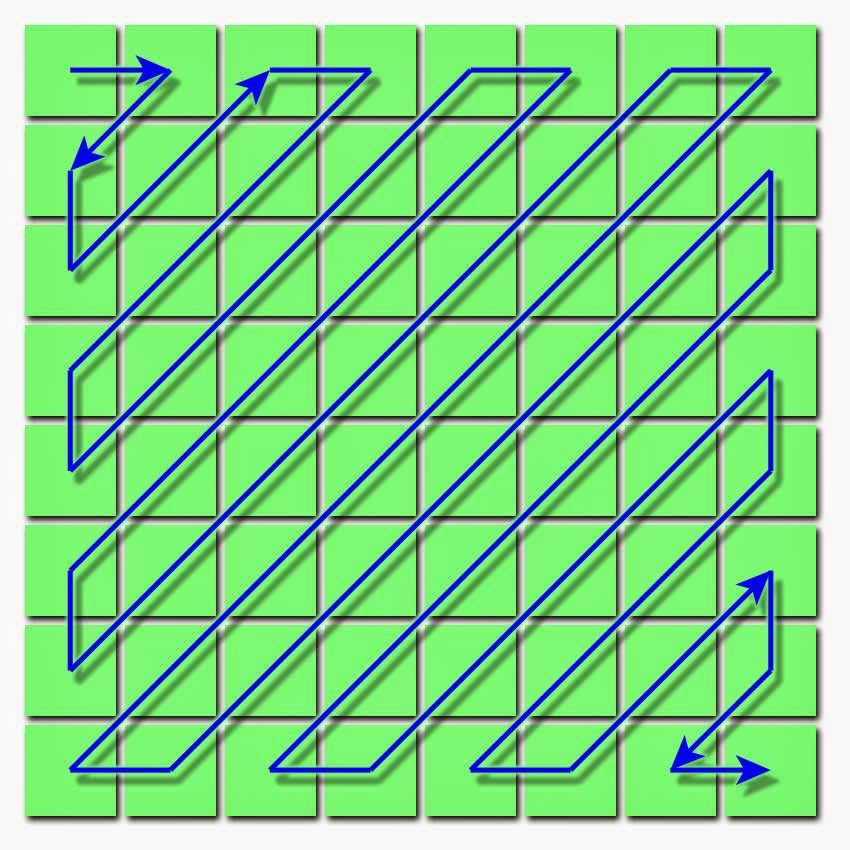
\includegraphics[width=\linewidth]{./figures/zigzag.jpg}
\caption{Path of the pointer~\autocite{dctProcessing}}
\end{wrapfigure}

The result of this transformation is a 64 integer long string.
Most of the integers with be repeated.
JFIF performs run length encoding to losslessly compress the string.
It does this by representing each integer as two values, the \texttt{integer} and the \texttt{amount of time it is repeated}.
For a string with many repetitions, run length encoding can reduce the space required to the data drastically.

\subsection{Huffman Coding}\label{huffman}
To convert the string of data into binary, huffman coding is performed.
Huffman coding furthers losslessly compresses the data by effectively assigning symbols to each element in the string.
Firstly, an huffman tree is created from the string.

To create an huffman tree, the frequency of every element is counted.
% Finish this once you understand it better!!!

\newpage
\printbibliography

\end{document}
